\documentclass[a4paper, 12pt]{article}
\usepackage{amsmath}
\usepackage{color}
\usepackage{dsfont}
\usepackage[utf8]{inputenc}
\usepackage{graphicx}
\usepackage[left=2cm, right=2cm, bottom=3cm, top=2cm]{geometry}
\usepackage{microtype}
\usepackage{natbib}
\usepackage{pdflscape}


\definecolor{orange}{rgb}{1, 0.5, 0}
\definecolor{green}{rgb}{0, 0.5, 0}

\newcommand{\hypers}{\boldsymbol{\alpha}}
\newcommand{\params}{\boldsymbol{\theta}}
\newcommand{\data}{\boldsymbol{d}}
\newcommand{\info}{I}
\newcommand{\x}{x}
\newcommand{\todo}{\color{orange} \bf}


\title{Crystals}
\author{Brendon J. Brewer}
\date{}

\begin{document}
\maketitle

%\abstract{\noindent Abstract}

% Need this after the abstract
\setlength{\parindent}{0pt}
\setlength{\parskip}{8pt}

\section{Bayesian inference}
In the Bayesian framework
\citep{gregory2005bayesian, o2004kendall, sivia2006data},
probability distributions are used to model
states of uncertainty about the values of unknown quantities.
Typically, one starts with the ``prior distribution''
for unknown quantities (`parameters') $\params$, written $p(\params | \info)$
(the probability distribution for $\params$ {\em given} prior information
$\info$). This is supplemented with $p(\data | \params, \info)$,
which describes the uncertainty about the data which we {\em would} have,
if we knew the parameters (and the prior information), as a function of
the parameters. This describes uncertainty about what data will be observed,
but knowledge about the fact that the data has something to do with the
parameters $\params$.
The
product of these two distributions is the joint prior
\begin{align}
p(\params, \data | \info) &= p(\params | \info)p(\data | \params, \info)
\end{align}
which describes uncertainty about the value of both the parameters and the
dataset.

Once a specific observed dataset $\data_o$ is known, knowledge about
$\params$ is updated from the prior to the posterior
\begin{align}
p(\params | \data_0, \info) &\propto
    p(\params | \info)p(\data_o | \params, \info).
\end{align}
which takes the specific data $\data_0$ into account. With a specific dataset
$\data_0$ being specified, $p(\data_o | \params,\info)$ is a function of the
unknown parameters $\params$ and is called the {\em likelihood function}.
The posterior distribution is therefore proportional to the prior distribution
times the likelihood function.

When $\params$ is a large collection of parameters, the posterior distribution
is a probability distribution over a high-dimensional parameter space. To
represent it computationally, Markov Chain Monte Carlo (MCMC) methods are
often used to generate samples from the parameter space, according to the
posterior distribution. The output is a collection of plausible values of the
parameters which can be used to approximate posterior probabilities.
For example, the probability some parameter $\theta$ is greater than 3.4
is approximately the proportion of the posterior samples that have
$\theta > 3.4$.

We compute the posterior distribution for the unknown parameters of the
components, using \citep{dnest4} to generate samples from that posterior
distribution.

\section{The model curve}
The algorithm fits the data with a model curve
$f(\x)$, defined between $\x=\x_{\rm min}$ and $\x=\x_{\rm max}$,
which is assumed to be a sum of the following components:
\begin{enumerate}
\item A background component, described by parameters $\params_{\rm bg}$
\item A wide component, described by parameters $\params_{\rm wide}$
\item Narrow spikes, described by parameters $\params_{\rm narrow}$
\end{enumerate}

The total model function $f_{\rm tot}(x)$ is therefore
\begin{align}
f_{\rm tot}(\x) &= f_{\rm bg}(\x; \params_{\rm bg})
       + f_{\rm wide}(\x; \params_{\rm wide})
       + f_{\rm narrow}(\x; \params_{\rm narrow})
\end{align}
and the crystallinity is defined as the proportion of the area in the
wide and narrow components which is accounted for by the wide component:
\begin{align}
C &= \frac{\int_{\x_{\rm min}}^{\x_{\rm max}}
            f_{\rm wide}(\x; \params_{\rm wide}) \, d\x}
          {\int_{\x_{\rm min}}^{\x_{\rm max}}
            \left[f_{\rm wide}(\x; \params_{\rm wide})
            + f_{\rm narrow}(\x; \params_{\rm narrow}) \right] \, d\x}
\end{align}



From each sample,
it is possible to compute the crystallinity, making it straightforward to
calculate the marginal posterior distribution of the crystallinity, describing
the remaining uncertainty about its value in the light of the data.

In the following subsections, I describe the specific parameterisations of the
three parts of the model curve.

\subsection{The background component}
The background component is assumed to be piecewise linear
{\todo between $\x=\x_{\rm min}$ and $\x=10$, between $\x=10$ and $\x=40$,
and between $\x=40$ and $\x=\x_{\rm max}$}.
We parameterise the background component using
five parameters. Firstly, there is a mean level $b$, which sets the
typical amplitude of the background component. There are also four parameters
$n_1, ..., n_4$, which set the positions of four control points:
\begin{align}
\left(\x_{\rm min}, be^{n_1}\right) \nonumber\\
\left(10, be^{n_2}\right) \nonumber\\
\left(40, be^{n_3}\right) \nonumber\\
\left(\x_{\rm max}, be^{n_4}\right) \nonumber
\end{align}
The value of the background component at any other point is found by
linear interpolation. Figure~\ref{fig:background} shows three example
background curves generated from this parameterisation, with typical
values of the parameters.

\begin{figure}
\centering
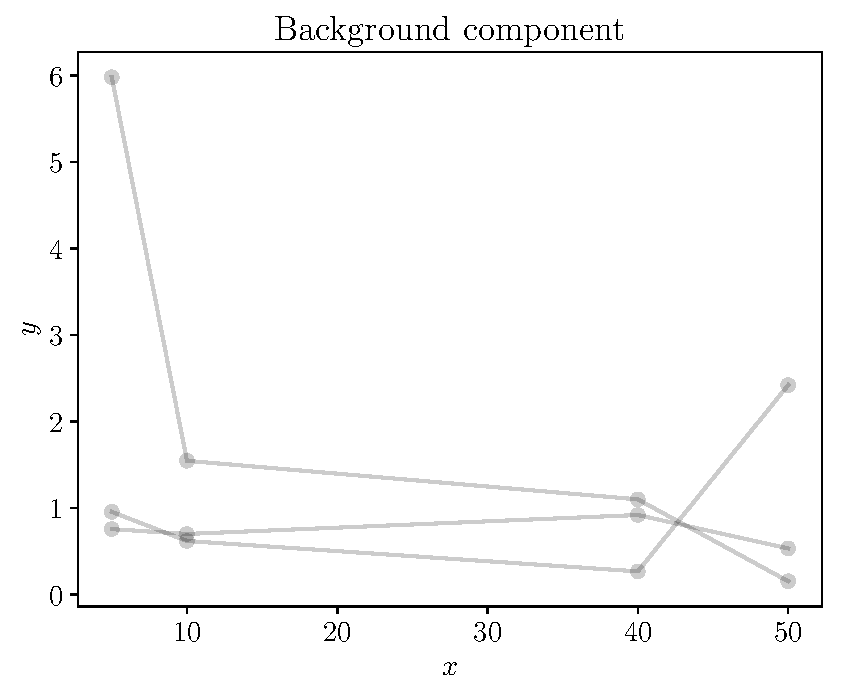
\includegraphics[width=0.7\textwidth]{figures/background.pdf}
\caption{\it Three example functions showing possible shapes of the
background component.\label{fig:background}}
\end{figure}

\subsection{The narrow spikes}
I assumed that there is some number $N_{\rm narrow}$ of narrow spikes,
each of which has a gaussian shape. The $i$th narrow spike is parameterised
by its central position $X_{i, \rm narrow}$,
amplitude $A_{i, \rm narrow}$, and width $A_{i, \rm narrow}$.
The parameter vector for narrow spikes is
\begin{align}
\params_{\rm narrow} &=
  \{N_{\rm narrow}, X_1, X_2, ..., X_{N, \rm narrow},
    A_1, A_2, ..., A_{N, \rm narrow},
    W_1, W_2, ..., W_{N, \rm narrow}\}
\end{align}
and the total shape contributed by the
narrow spikes is a sum of the $N_{\rm narrow}$ gaussians:
\begin{align}
f_{\rm narrow}(\x; \params_{\rm narrow}) &=
    \sum_{i=1}^{N_{\rm narrow}} A_{i, \rm narrow}
 \exp\left[-\frac{1}{2W_{i, \rm narrow}^2}\left(x - X_{i, \rm narrow}\right)^2\right].
\end{align}

\subsection{The wide component}
The wide component is also composed of gaussians, like the narrow spikes.
In fact, the only real difference is the prior distributions for the positions,
amplitudes, and widths, given in Section~\ref{sec:priors}.

There is some number $N_{\rm wide}$ of gaussians in the wide component.
The $i$th gaussian is parameterised
by its central position $X_{i, \rm wide}$,
amplitude $A_{i, \rm wide}$, and width $A_{i, \rm wide}$.
The parameter vector for wide gaussians is
\begin{align}
\params_{\rm wide} &=
  \{N_{\rm wide}, X_1, X_2, ..., X_{N, \rm wide},
    A_1, A_2, ..., A_{N, \rm wide},
    W_1, W_2, ..., W_{N, \rm wide}\}
\end{align}
and the total shape contributed by the
wide component is a sum of the $N_{\rm wide}$ gaussians:
\begin{align}
f_{\rm wide}(\x; \params_{\rm wide}) &=
    \sum_{i=1}^{N_{\rm wide}} A_{i, \rm wide}
 \exp\left[-\frac{1}{2W_{i, \rm wide}^2}\left(x - X_{i, \rm wide}\right)^2\right].
\end{align}

Figure~\ref{fig:wide_component} shows several examples of plausible
wide component shapes.

\begin{figure}[!ht]
\centering
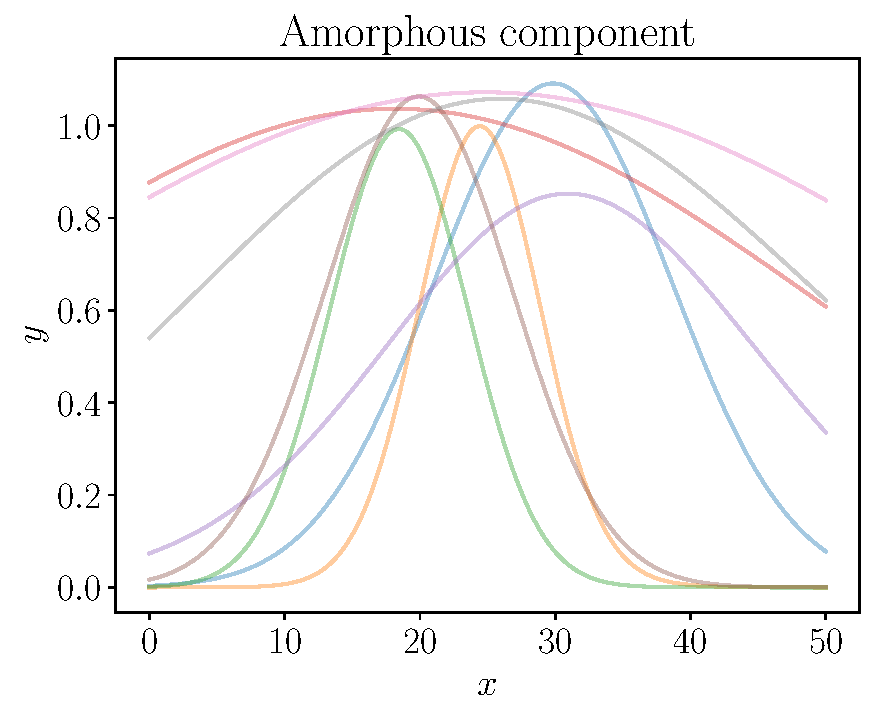
\includegraphics[scale=0.7]{figures/wide_component.pdf}
\caption{\it Some examples of plausible shapes for the wide component,
generated from the prior distribution for its parameters
(Section~\ref{sec:priors}). For visual purposes only, these
were scaled to amplitudes $\sim$ 1. \label{fig:wide_component}}
\end{figure}

\subsection{Derived properties}
Some derived properties of the wide component are used to summarise its shape.
We have included `skewness', which describes asymmetry, and `nongaussianity'
which quantifies the departure from gaussianity. These are not the same
concept, as the wide component could be non-gaussian while still being symmetric
(and thus having zero skewness).

Defining the normalised version of the wide component as
\begin{align}
g(\x) &= \frac{f_{\rm wide}(\x)}
             {\int_{-\infty}^\infty f_{\rm wide}(\x') \, d\x'},
\end{align}
its center of mass by
\begin{align}
\textnormal{center} &= \int_{-\infty}^\infty x g(\x) \, d\x,
\end{align}
and its width (second central moment) by
\begin{align}
\textnormal{width} &= \sqrt{\int_{-\infty}^\infty
                            g(\x) \left(\x - \textnormal{center}\right)^2
                            \, d\x},
\end{align}
the skewness is
\begin{align}
\textnormal{skewness} &= \int_{-\infty}^\infty
                           g(\x) 
                           \left(
                             \frac{x - \textnormal{center}}{\textnormal{width}}
                           \right)^3
                         \, d\x.
\end{align}

To quantify the non-gaussianity, we construct a gaussian
$g'(\x)$
with the same centre, width, and total integral as $g(\x)$, and compute the
Kullback-Leibler divergence from $g'$ to $g$:
\begin{align}
\textnormal{non-gaussianity} &= 
    \int_{-\infty}^\infty g(\x) \log\left[\frac{g(\x)}{g'(\x)}\right] \, d\x.
\end{align}
where
\begin{align}
g'(\x) &= \frac{1}{\textnormal{width} \times \sqrt{2\pi}}
            \exp\left[-\frac{1}{2\times (\textnormal{width})^2}
                    \left(\x - \textnormal{center}\right)^2\right].
\end{align}
The Kullback-Leibler divergence is a standard way of quantifying how
different one measure is from another \citep{knuth2012foundations}.
It is zero when the two measures are the same, in our case,
if $g(\x)$ is a gaussian.

See Figures~\ref{fig:skewness} and~\ref{fig:nongaussianity} for example
shapes for the wide component, and corresponding values of the skewness
and nongaussianity.

\begin{figure}[!ht]
\centering
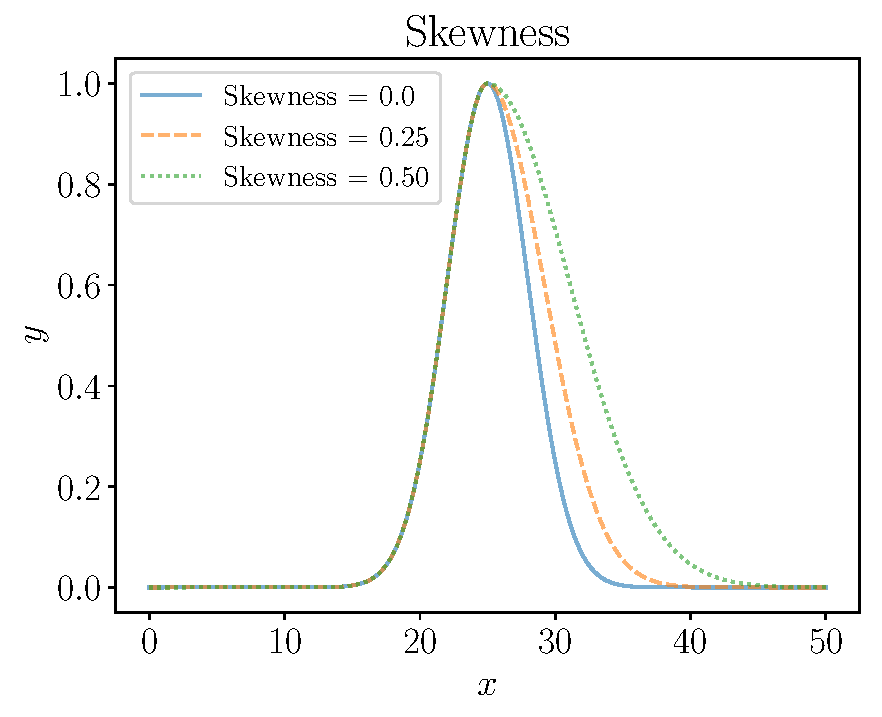
\includegraphics[scale=0.7]{figures/skewness.pdf}
\caption{\it Examples of wide component shapes with different values
for the skewness.\label{fig:skewness}}
\end{figure}

\begin{figure}[!ht]
\centering
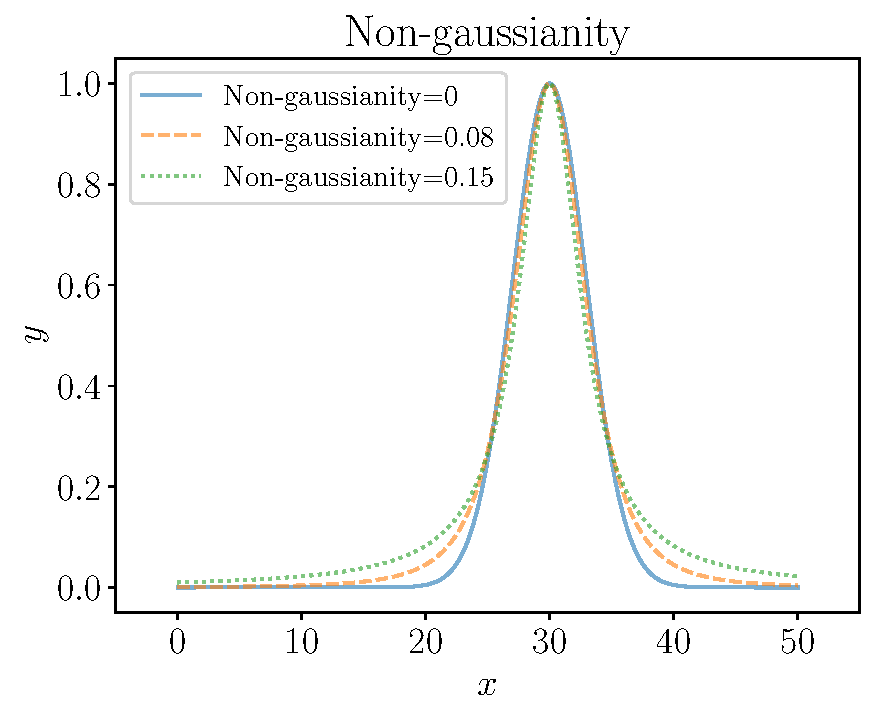
\includegraphics[scale=0.7]{figures/nongaussianity.pdf}
\caption{\it Examples of wide component shapes with different values
for the nongaussianity.\label{fig:nongaussianity}}
\end{figure}

\section{Prior probability distributions}\label{sec:priors}
The joint prior distribution for the hyperparameters, parameters, and data,
is written $p(\hypers, \params, \data | \info)$, and is usually factorised
in this way:
\begin{align}
p(\hypers, \params, \data | \info) &=
    p(\hypers | \info)p(\params | \hypers, \info)
    p(\data | \params, \hypers, \info)\\
    &= p(\hypers | \info)p(\params | \hypers, \info)
    p(\data | \params, \info)
\end{align}
where the first step is true in general by the product rule, and the second
step assumes that knowing the parameters would make the hyperparameters
irrelevant when predicting what data would be observed.

All of the assumptions are given in Table~\ref{tab:priors}.

\begin{landscape}

\begin{table}
\footnotesize
\centering
\begin{tabular}{|lll|}
\hline
{\bf Quantity}      &   {\bf Meaning}   &  {\bf Prior distribution}\\
\hline
{\em Prior information}&&\\
\hline
$n$ & Number of measurements & given\\
$\{\x_1, \x_2, ..., \x_n\}$  & $\x$-values of measurements & given \\
\hline
{\em Hyperparameters} & &\\
$N_{\rm narrow}$   &   Number of narrow spikes    &  $\propto 1/(N_{\rm narrow}+1)$, $N_{\rm narrow} \in \{0, 1, ..., 300\}$ \\
$N_{\rm wide}$   &   Number of wide spikes    &  $\propto 1/(N_{\rm wide}+1)$,
$N_{\rm wide} \in \{0, 1, ..., 300\}$ \\
$a_{\ln A, \rm narrow}$ & Typical log-amplitude of narrow spikes & Laplace(0, 5)\\
$a_{\ln A, \rm wide}$ & Typical log-amplitude of wide spikes & Laplace(0, 5)\\
$b_{\ln A, \rm narrow}$ & Diversity of log-amplitude of narrow spikes & Uniform(0, 5)\\
$b_{\ln A, \rm wide}$ & Diversity of log-amplitude of wide spikes & Uniform(0, 5)\\
$a_{\ln W, \rm narrow}$ & Typical log-width of narrow spikes & LogUniform$(10^{-3}x_{\rm range}, 0.05x_{\rm range})$\\
$a_{\ln W, \rm wide}$ & Typical log-width of wide spikes & LogUniform$(0.05x_{\rm range}, x_{\rm range})$\\
$b_{\ln W, \rm narrow}$ & Diversity of log-width of narrow spikes & Uniform(0, 0.1)\\
$b_{\ln W, \rm wide}$ & Diversity of log-width of wide spikes & Uniform(0, 0.2)\\
\hline
{\em Background parameters}&&\\
$b$       & Mean background level       & $\ln b \sim $ Laplace$(0, 5)$\\
$\{n_1, ..., n_4\}$  & Background deviations & iid Normal$(0,1)$\\
\hline
{\em Narrow spike parameters}&&\\
$X_{i, \rm narrow}$ & Positions of narrow spikes &
                            Uniform$(x_{\rm min}, x_{\rm max})$ \\
$A_{i, \rm narrow}$ & Amplitudes of narrow spikes &
 $\ln A_{i, \rm narrow} \sim \textnormal{Laplace}\left(a_{\ln A, \rm narrow}, b_{\ln A, \rm narrow}\right)$ \\
$W_{i, \rm narrow}$ & Widths of narrow spikes &
 $\ln W_{i, \rm narrow} \sim \textnormal{Laplace}\left(a_{\ln W, \rm narrow}, b_{\ln W, \rm narrow}\right)$ \\
\hline
{\em Wide spike parameters}&&\\
$X_{i, \rm wide}$ & Positions of wide spikes &
          Uniform$(x_{\rm min}+0.3x_{\rm range}, x_{\rm max}-0.3x_{\rm range})$ \\
$A_{i, \rm wide}$ & Amplitudes of wide spikes &
 $\ln A_{i, \rm wide} \sim \textnormal{Laplace}\left(a_{\ln A, \rm wide}, b_{\ln A, \rm wide}\right)$ \\
$W_{i, \rm wide}$ & Widths of wide spikes &
 $\ln W_{i, \rm wide} \sim \textnormal{Laplace}\left(a_{\ln W, \rm wide}, b_{\ln W, \rm wide}\right)$ \\
\hline
{\em Noise parameters}&&\\
$\sigma_0$ &    Constant noise level  &   $\ln \sigma_0 \sim \textnormal{Laplace}(0,5)$\\
$\sigma_1$ &    Noise proportionality   &  $\ln \sigma_1 \sim \textnormal{Laplace}(0,5)$ \\
$\nu$     &   Shape parameter for residuals   &   LogUniform$(1, 1000)$\\
\hline
{\em Data}&&\\
\hline
$\{y_1, y_2, ..., y_n\}$  &   Measurements    & iid Student-$t(f(x_i; \params), ,\nu)$\\
\hline
\end{tabular}
\caption{\it The prior distributions for all hyperparameters,
parameters, and the data.\label{tab:priors}}
\end{table}

\end{landscape}

The Laplace, or biexponential, distribution with location parameter
(central position) $a$ and scale parameter (width) $b$ has probability
density given by
\begin{align}
p(x | a, b) &= \frac{1}{2b}\exp\left[-\frac{|x - a|}{b}\right].
\end{align}
We used a Laplace distribution for informative priors, rather than
a more conventional normal distribution, because it assigns higher
prior probability to values far from the center, and can be computed conveniently, i.e., no special functions such as {\tt erf} are needed
to compute the cumulative distribution function.

\section{Installation and usage}

\subsection*{Windows}
The entire repository, including C++ and Python source code, and a Windows
executable, is hosted on Bitbucket. The URL for the git repository is

{\tt https://bitbucket.org/eggplantbren/crystals}

If you do not use git, the repository can simply be downloaded from

{\tt https://bitbucket.org/eggplantbren/crystals/get/c78decf570f0.zip}

and unzipped into any location on your computer.


\bibliographystyle{plainnat}
\bibliography{references}

\end{document}

